
%
% midterm, solutions ecs222A -- fall 98
%
\documentclass[11pt]{article}
\usepackage{amsmath}
\usepackage{graphicx}
\usepackage{listings}
\usepackage{caption}
\usepackage{subcaption}
\usepackage{amsfonts}
\newcommand{\tf}{{\hfill\fbox{{\large\bf True}}\qquad\fbox{{\large\bf False}}}}
\newcommand{\bfit}[1]{{\textbf{\textit{#1}}}}
% to be \input after \documentstyle[11pt,twoside]{article}

% page size parameters

\setlength\itemindent{0.1in}
\setlength{\itemsep}{0in}

\setlength{\topmargin}{0in}
\setlength\oddsidemargin{0in}
\setlength\evensidemargin{0in}
\setlength\parindent{0.0in} 
\setlength\textwidth{6.5in}
\setlength\textheight{8.5in}
\setlength{\parskip}{\medskipamount}

\newenvironment{newmath}{\begin{displaymath}%
\setlength{\abovedisplayskip}{4pt}%
\setlength{\belowdisplayskip}{4pt}%
\setlength{\abovedisplayshortskip}{3pt}%
\setlength{\belowdisplayshortskip}{3pt} }{\end{displaymath}}

% Cross-references for handout numbers.

\makeatletter
\newcommand{\hlabel}[2]{\write\@auxout{\string\newlabel{#1}{{#2}{0}}}}
\makeatother

%\input{../../handouts}	% defines handout labels


% Make \section use \large instead of \Large typeface.

\makeatletter
\def\section{\@startsection {section}{1}{\z@}{-3.25ex plus -1ex minus -.2ex}
{1.5ex plus .2ex}{\large\bf}}
\makeatother




% use \nullsec if the first thing after \handout isn't \section

\newcommand{\nullsec}{\vspace*{3.25ex plus 1ex minus .2ex}}


% header hackery

\newlength{\toppush}
\setlength{\toppush}{2\headheight}
\addtolength{\toppush}{\headsep}


\def\subjnum{MAT 226B}
\def\subjname{Large-Scale Matrix Computations}

\def\doheading#1#2#3{\vfill\eject\vspace*{-\toppush}%
\vbox{\hbox to\textwidth{{\bf}\subjnum: \subjname \hfil Handout #1\strut}%
\hbox to\textwidth{UC Davis --- Minhao Cheng \hfil#3\strut}%
    \hrule}}

\newcommand{\htitle}[1]{\vspace*{3.25ex plus 1ex minus .2ex}%
  \begin{center}{\Large\bf #1}\end{center}}


% page style that displays just footers
\makeatletter
\def\ps@justfooters{\let\@mkboth\@gobbletwo\def\@oddhead{}%
	\def\evenhead{}}
\makeatother

% \handout{handout label}{title}{date}

\newcommand{\handout}[3]{\thispagestyle{justfooters}%
  \markboth{\subjnum\ Handout \protect\ref{#1}: #2}%
    {\subjnum\ Handout \protect\ref{#1}: #2}%
  \pagestyle{myheadings}%
  \doheading{\protect\ref{#1}}{#2}{#3}%
  \htitle{#2}}


% \handoutwithouttitle{handout label}{date}

\newcommand{\handoutwithouttitle}[2]{\thispagestyle{justfooters}%
  \markboth{\subjnum\ Handout \protect\ref{#1}}%
    {\subjnum\ Handout \protect\ref{#1}}%
  \pagestyle{myheadings}%
  \doheading{\protect\ref{#1}}{#2}{}}


% hack to get (over) on the bottom of all following odd pages
% must be placed by hand in source text

\makeatletter
\outer\def\OVER{\def\@oddfoot{\message{OVER}\rm\hfil(over)}}
\makeatother

\newcommand{\from}{{from}}


\begin{document}
\handout{midterm}{Final Project }{March 13 2016}

%%%%%%%%%%%%%%%%%%%%%%%%%%%%%%%%%%%%%%%%%%%%%%%%%%%%%%%%%%%%%%%%%%%%%%%%

\section{Problem 1}
{\bf(a)} After k steps Arnoldi process, we got $V_k, H_k$. Then $AV_k=V_kH_k+h_{k+1,k}v_{k+1}e_k^T$. From above, when $R=r \in \mathbb{C}$, since $r=R$ and $\beta=||r||_2$, $M^jR=||R||_2M^jV_ke_1=||r||_2V_kH_k^je_1=\beta V_kH_k^je_1$\\
{\bf(b)} 
We use Taylor expansion at $s_0$ and get
\begin{equation}
	Z(s)=\sum\limits_{j=k-1}^\infty(s-s_0)^jM_j 
\end{equation}
where $M_j=C^TM^jR$, Same, we can get
\begin{equation}
Z_k(s)=\sum\limits_{j=k-1}^\infty(s-s_0)^jM_j^{(k)} 
\end{equation}
where $M_j^{(k)} =C_k^HH_k^j\beta e_1$\\
From (1),(2) and (a), we can get
\begin{equation*}
	\begin{split}
	Z(s)-Z_k(s)&=\sum\limits_{j=k-1}^\infty(s-s_0)^j(M_j-M_j^{(k)})\\
	&=\sum\limits_{j=k-1}^\infty(s-s_0)^j(C^TM^jR-C^HV_kH_k^j\beta e_1)\\
	&= \sum\limits_{j=k-1}^\infty(s-s_0)^j(C^T-C^H)M^jR\\
	&=O((s-s_0)^k)
	\end{split}
\end{equation*}

Therefore, $Z(s)=Z_k(s)+O((s-s_0)^k)$
 \\

\section{Problem 2}
\begin{lstlisting}
function [Q,H] = arnoldi(A,q1,m)
n = length(A);
if nargin < 3, m = n; end
q1 = q1/norm(q1);
Q = zeros(n,m); 
Q(:,1) = q1;
H = zeros(m+1,m);
for k=1:m
	z = A*Q(:,k);
	for i=1:k
		H(i,k) = Q(:,i)'*z;
		z = z - H(i,k)*Q(:,i);
	end
	if k < n
		H(k+1,k) = norm(z);
	if H(k+1,k) == 0, return, end
		Q(:,k+1) = z/H(k+1,k);
	end
end
H=H(1:m,1:m);
Q=Q(1:n,1:m);
end
\end{lstlisting}


\section{Problem 3}
{\bf (a)}	When $A=A^H$, we can choose $c=\bar{r}$ in the nonsymmetric lanczos algorithms. And therefore, $w_n=\bar{v_n}$ for all n. Thus, instead doing two matrix-vector multiplication in then nonsymmetric lanczos case, we can only do once. That is to say, we needn't calculate $s, \gamma$. Therefore, each matrix vector product with $A^T$ can be replaced by a matrix vector multiplication with J. Therefore, it saved half calculating time and space. When $A^TJ=JA$, we can use the same idea as before.  We set $c=\frac{Jr}{||r||}$ then $w_1=\frac{c}{||c||}=\frac{Jv_1}{||Jv_1||}$. In the later iteration, $w_n=\frac{Jv_n}{|||Jv_n||}$. Therefore, as before, it saved half calculating time and space.\\
{\bf (b)}  When $A^HJ=JA=J^HA=(A^HJ)^H$, we can use the same idea as before.  We set $c=\frac{Jr}{||r||}$ then $w_1=\frac{c}{||c||}=\frac{Jv_1}{||Jv_1||}$. In the later iteration, $w_n=\frac{Jv_n}{|||Jv_n||}$. Therefore, as before, it saved half calculating time and space.  \\

\section{Problem 4}
\subsection{Plots of Z and Zk}
In the "example1" dataset, we choose s0=f_max, when k=130, it convergence. The result of $Z_k^{(1,1)}(s)$ for both nonsymmetric lanczos and Arnoldi algorithms and the exact result of $Z^{(1,1)}(s)$ are as follows:\\
\begin{figure}
	\centering
	\begin{subfigure}{.3\textwidth}
		\centering
		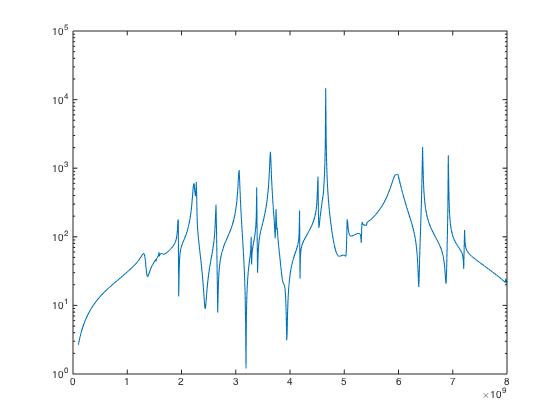
\includegraphics[width=1\linewidth]{lanzk11}
		\caption{Lanczos: Zk(1,1)}
	\end{subfigure}
	\begin{subfigure}{.3\textwidth}
		\centering
		\includegraphics[width=1\linewidth]{arnoldiz11}
		\caption{Arnoldi: Zk(1,1)}
	\end{subfigure}
	\begin{subfigure}{.3\textwidth}
			\centering
			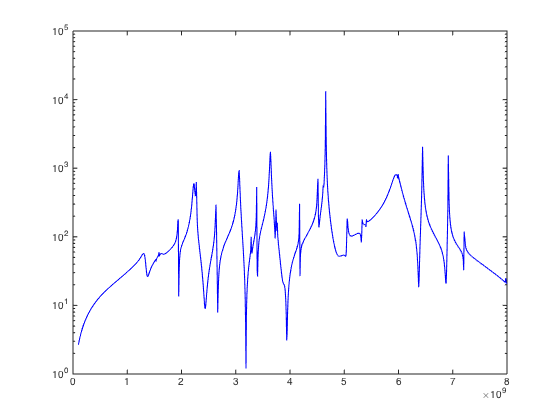
\includegraphics[width=1\linewidth]{exactzk11}
			\caption{Z(1,1))}
	\end{subfigure}
\end{figure}
 The result of $Z_k^{(1,2)}(s)$ for both nonsymmetric lanczos and Arnoldi algorithms and the exact result of $Z^{(1,2)}(s)$ are as follows:\\
\begin{figure}
	\centering
	\begin{subfigure}{.3\textwidth}
		\centering
		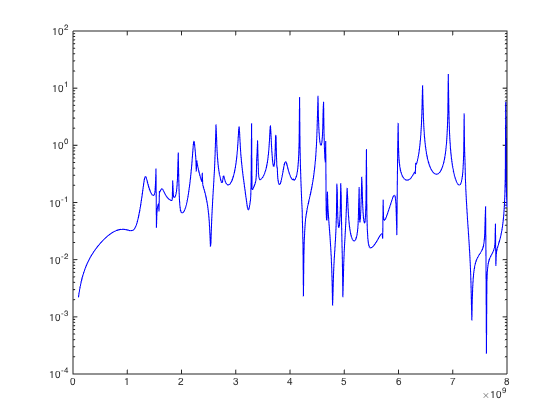
\includegraphics[width=1\linewidth]{lanzk12}
		\caption{Lanczos: Zk(1,2)}
	\end{subfigure}
	\begin{subfigure}{.3\textwidth}
		\centering
		\includegraphics[width=1\linewidth]{arnoldiz12}
		\caption{Arnoldi: Zk(1,2)}
	\end{subfigure}
	\begin{subfigure}{.3\textwidth}
		\centering
		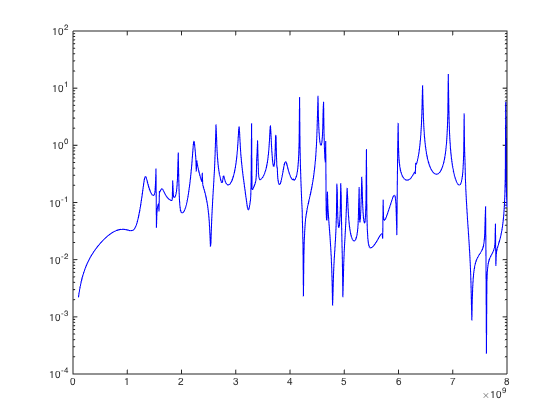
\includegraphics[width=1\linewidth]{exactzk12}
		\caption{Z(1,2)}
	\end{subfigure}
\end{figure}
The result of $Z_k^{(2,2)}(s)$ for both nonsymmetric lanczos and Arnoldi algorithms and the exact result of $Z^{(2,2)}(s)$ are as follows:\\
\begin{figure}
	\centering
	\begin{subfigure}{.3\textwidth}
		\centering
		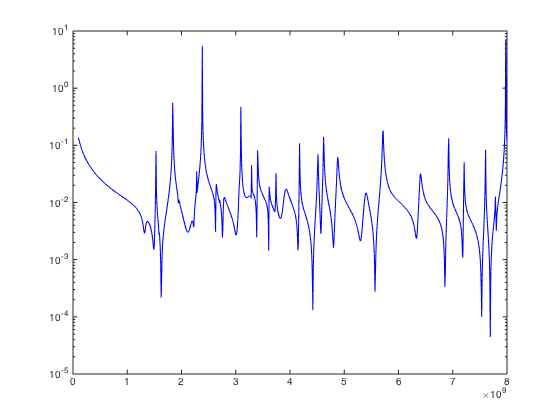
\includegraphics[width=1\linewidth]{lanzk22}
		\caption{Lanczos: Zk(2,2)}
	\end{subfigure}
	\begin{subfigure}{.3\textwidth}
		\centering
		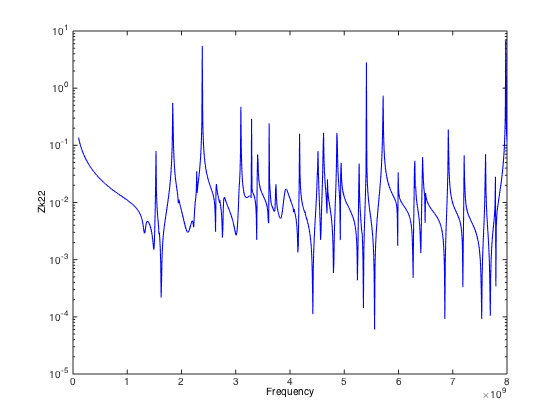
\includegraphics[width=1\linewidth]{arnoldizk22}
		\caption{Arnoldi: Zk(2,2)}
	\end{subfigure}
	\begin{subfigure}{.3\textwidth}
		\centering
		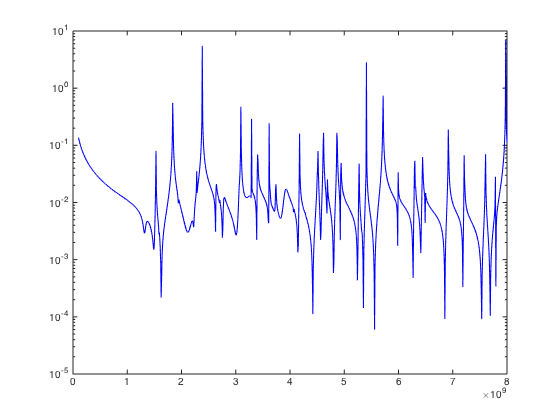
\includegraphics[width=1\linewidth]{exactzk22}
		\caption{Z(2,2)}
	\end{subfigure}
\end{figure}
The result of $Z_k^{(2,3)}(s)$ for both nonsymmetric lanczos and Arnoldi algorithms and the exact result of $Z^{(2,3)}(s)$ are as follows:
\begin{figure}
	\centering
	\begin{subfigure}{.3\textwidth}
		\centering
		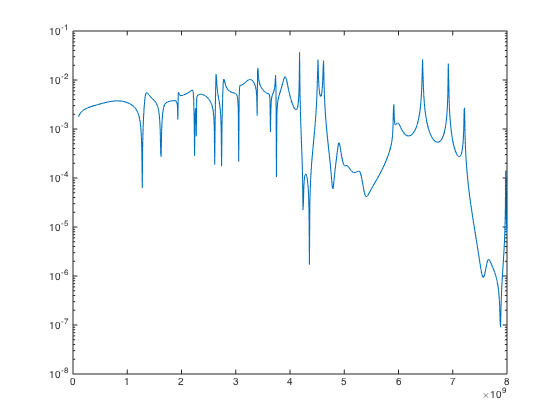
\includegraphics[width=1\linewidth]{lanzk23}
		\caption{Lanczos: Zk(2,3)}
	\end{subfigure}
	\begin{subfigure}{.3\textwidth}
		\centering
		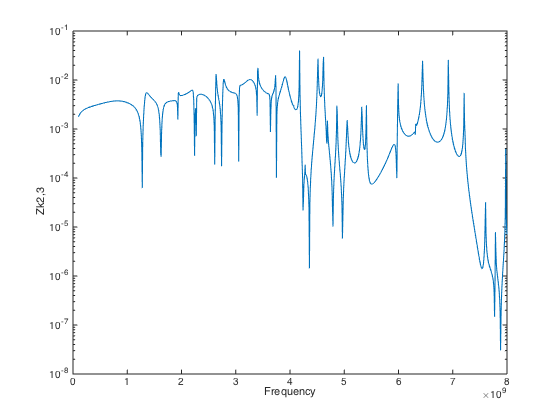
\includegraphics[width=1\linewidth]{arnoldizk23}
		\caption{Arnoldi: Zk(2,3)}
	\end{subfigure}
	\begin{subfigure}{.3\textwidth}
		\centering
		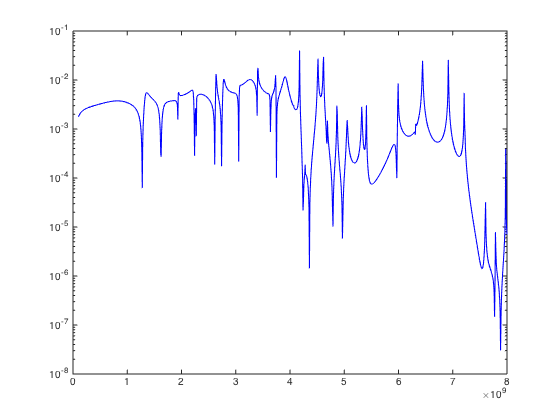
\includegraphics[width=1\linewidth]{exactzk23}
		\caption{Z(2,3)}
	\end{subfigure}
\end{figure}

\subsubsection{Choise of S0}
 In "example1"\&"example2" data, since we can get the exact number of Z, therefore,  when the difference between $Z_k$ and Z is less than 1\% of $Z$, it is a good approximation of $Z$.
%%%%%%%%%%%%%%%%%%%%%%%%%%%%%%%%%%%%%%%%%%%%%%%%%%%%%%%%%%%%%%%%%%%%%%%%




%%%%%%%%%%%%%%%%%%%%%%%%%%%%%%%%%%%%%%%%%%%%%%%%%%%%%%%%%%%%%%%%%%%%%%%%%%%%


\end{document}

@
